\section{Logische Gatter}

	\subsection{Verhalten logischer Gatter}
		\begin{multicols}{2}
			\subsubsection{St"orabstand}
				High-Pegel: $ U_{n_H} = U_{a_Hmin} - U_{e_Hmin} $\\
				Low-Pegel: $ U_{n_L} = U_{e_Lmax} - U_{a_Lmax} $\\
				
		%\end{multicols}

		%\begin{multicols}{2}
			\subsubsection{Propagation delay (Verz"ogerungszeit) }
				Zeit zwischen 50\% von $V_{max}$ am Eingang und 50\% von $V_{max}$ am Ausgang.\\
				$t_{pd}=\frac{t_{p_{LH}}+t_{p_{HL}}}{2}$\\
				
			\subsubsection{Transition time (Übergangszeit)}
				Zeit zwischen 10\% und 90\% von $V_{max}$.\\
				$t_{t_{LH}}$: Transition time low to high.\\
				$t_{t_{HL}}$: Transition time high to low.\\
				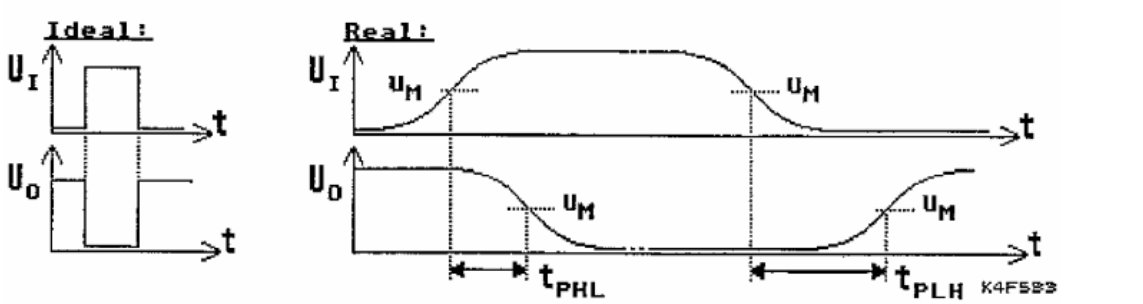
\includegraphics[width=0.2\textwidth]{pics/delay}
				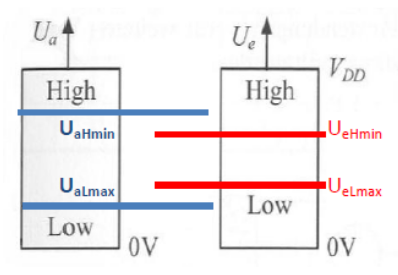
\includegraphics[width=0.2\textwidth]{pics/Pegelbereiche_Stoerabstand}
		\end{multicols}

\subsection{Hazards}
\begin{tabular}{rp{5cm}p{1cm}rp{5cm}}
	\textbf{statisch:}&kurzzeitige Änderung, obwohl keine Änderung gegeben ist.&&
	\textbf{dynamisch:}&mehrere Änderungen, obwohl nur eine Änderung gegeben ist.\\
\end{tabular}\\
\textbf{Vermeiden von Hazards:} Redundante Schaltungselemente einfügen (Fielen bei KV-Diagramm weg)
		


%\newpage
\begin{sidewaystable}
\subsection{Aufbau logischer Gatter}
\begin{tabular}{|c|c|c|c|c|c|c|c|c|}
\hline
Funktion & Buffer & NOT & AND & NAND & OR & NOR & EXOR & XNOR\\
& & Nicht & Und & Nicht Und & Oder & Nicht Oder & Exklusiv Oder & Nicht Ex. Oder\\
& & Inverter & Konjunktion & & Disjunktion & & Antivalenz & "Aquivalenz \\
\hline
Formel & a & $ \overline a $ & $ a \cdot b $ & $ \overline{a \cdot b} $ & $ a + b $ & $ \overline{a + b} $ & $ a \oplus b $ & $ \overline{a \oplus b} $\\
& a & $ \overline a $ & $ a \wedge b $ & $ \overline{a \wedge b} $ & $ a \vee b $ & $ \overline{a \vee b} $ & $ a \not= b $ & $ \overline{a \not= b} $ \\
& a & !a & $ a \& b $ & $ !(a \& b) $ & a\#b & !(a\#b) & a\$b & !(a\$b) \\
\hline
& & & & & & & &\\
& 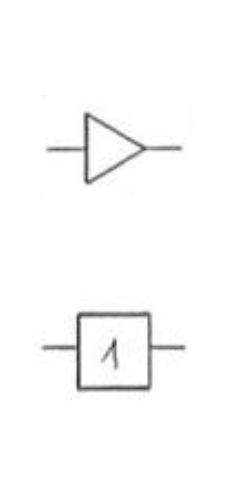
\includegraphics[width=0.08\textwidth]{pics/gates_symbol/buffer} & 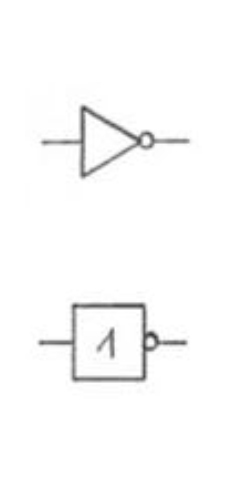
\includegraphics[width=0.08\textwidth]{pics/gates_symbol/not} & 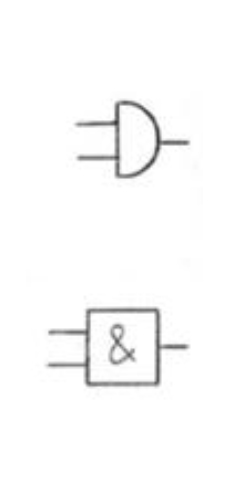
\includegraphics[width=0.08\textwidth]{pics/gates_symbol/and} & 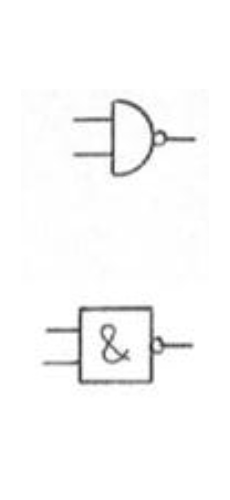
\includegraphics[width=0.08\textwidth]{pics/gates_symbol/nand} & 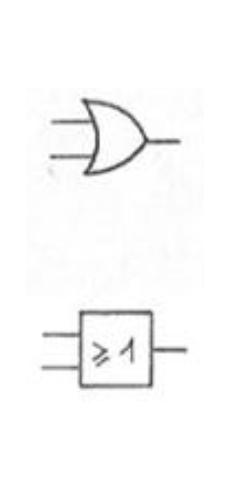
\includegraphics[width=0.08\textwidth]{pics/gates_symbol/or} & 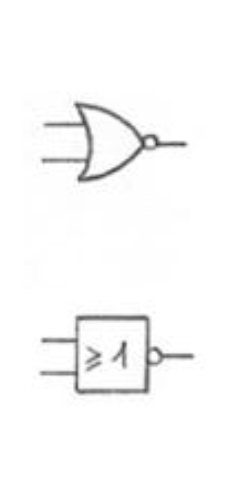
\includegraphics[width=0.08\textwidth]{pics/gates_symbol/nor} & 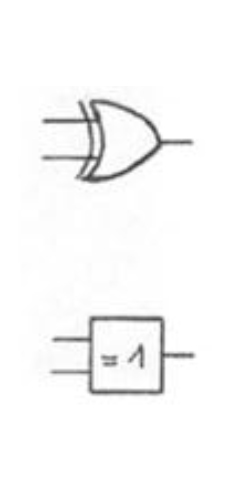
\includegraphics[width=0.08\textwidth]{pics/gates_symbol/exor} & 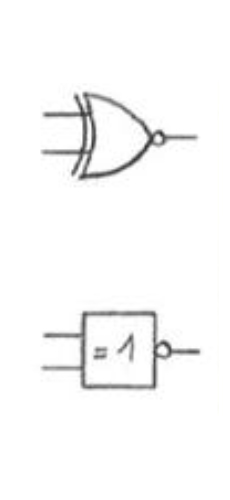
\includegraphics[width=0.08\textwidth]{pics/gates_symbol/xnor} \\
\hline
(0,0) & 0 & 1 & 0 & 1 & 0 & 1 & 0 & 1\\
(0,1) &   &   & 0 & 1 & 1 & 0 & 1 & 0\\
(1,0) & 1 & 0 & 0 & 1 & 1 & 0 & 1 & 0\\
(1,1) &   &   & 1 & 0 & 1 & 0 & 0 & 1\\
\hline
KDNF & \#(1) & \#(0) & \#(3) & \#(0,1,2) & \#(1,2,3) & \#(0) & \#(1,2) & \#(0,3) \\
KKNF & \&(0) & \&(1) & \&(0,1,2) & \&(3) & \&(0) & \&(1,2,3) & \&(0,3) & \&(1,2)\\
\hline
& & & & & & & &\\
& & 
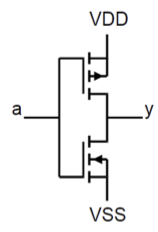
\includegraphics[width=0.12\textwidth]{pics/gates_schematic/inverter} & 
$ \overline{NAND} $ &
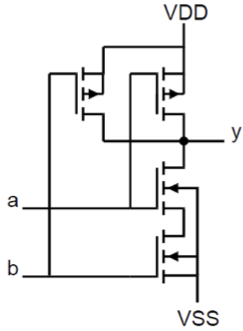
\includegraphics[width=0.12\textwidth]{pics/gates_schematic/NAND} &
$ \overline{NOR} $ &
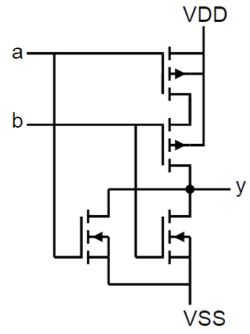
\includegraphics[width=0.12\textwidth]{pics/gates_schematic/NOR} & 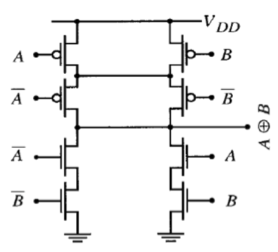
\includegraphics[width=0.12\textwidth]{pics/gates_schematic/XOR} & 
\\
\hline
\#Trans & & 2 & 6 & 4 & 6 & 4 & 8 & \\
\hline
\end{tabular}
\end{sidewaystable}